\def\mytitle{IDE ASSIGMNMENT}
\def\myauthor{MASEEDU NITIN}
\def\contact{massednitin@gmail.com}
\def\mymodule{Future Wireless Communications (FWC)}
\documentclass[journal,12pt,twocolumn]{IEEEtran}

\usepackage{setspace}
\usepackage{gensymb}
\usepackage{xcolor}
\usepackage{caption}
\usepackage[hyphens,spaces,obeyspaces]{url}
\usepackage[cmex10]{amsmath}
\usepackage{mathtools}
\singlespacing
\usepackage{amsthm}
\usepackage{mathrsfs}
\usepackage{txfonts}
\usepackage{stfloats}
\usepackage{cite}
\usepackage{cases}
\usepackage{subfig}
\usepackage{longtable}
\usepackage{multirow}
\twocolumn


\usepackage{graphicx}
\graphicspath{{./images/}}
\usepackage[colorlinks,linkcolor={black},citecolor={blue!80!black},urlcolor={blue!80!black}]{hyperref}
\usepackage[parfill]{parskip}
\usepackage{lmodern}
\usepackage{tikz}
\usepackage{circuitikz}
\usepackage{karnaugh-map}
\usepackage{pgf}
\usepackage[hyphenbreaks]{breakurl}

\usepackage{tabularx}
\usetikzlibrary{calc}
\newcommand{\brak}[1]{\left( #1 \right)}
\renewcommand*\familydefault{\sfdefault}
\usepackage{watermark}
\usepackage{lipsum}
\usepackage{xcolor}
\usepackage{listings}
\usepackage{float}
\usepackage{titlesec}
\DeclareMathOperator*{\Res}{Res}
\renewcommand\thesection{\arabic{section}}
\renewcommand\thesubsection{\thesection.\arabic{subsection}}
\renewcommand\thesubsubsection{\thesubsection.\arabic{subsubsection}}

\renewcommand\thesectiondis{\arabic{section}}
\renewcommand\thesubsectiondis{\thesectiondis.\arabic{subsection}}
\renewcommand\thesubsubsectiondis{\thesubsectiondis.\arabic{subsubsection}}
\titlespacing{\subsection}{1pt}{\parskip}{3pt}
\titlespacing{\subsubsection}{0pt}{\parskip}{-\parskip}
\titlespacing{\paragraph}{0pt}{\parskip}{\parskip}
\newcommand{\figuremacro}[5]{
    \begin{figure}[#1]
        \centering
        \includegraphics[width=#5\columnwidth]{#2}
        \caption[#3]{\textbf{#3}#4}
        \label{fig:#2}
    \end{figure}
}

\lstset{
frame=single, 
breaklines=true,
columns=fullflexible
}

%\thiswatermark{\centering \put(400,-128.0){\includegrphics[scale=0.3]{logo}} }
\title{\mytitle}
\author{\myauthor\hspace{1em}\\\contact\\IITH\hspace{0.5em}-\hspace{0.6em}\mymodule}
\date{20-12-2022}
\def\inputGnumericTable{}                                 %%
\lstset{
%language=C,
frame=single, 
breaklines=true,
columns=fullflexible
}
 \begin{document}
%

\theoremstyle{definition}
\newtheorem{theorem}{Theorem}[section]
\newtheorem{problem}{Problem}
\newtheorem{proposition}{Proposition}[section]
\newtheorem{lemma}{Lemma}[section]
\newtheorem{corollary}[theorem]{Corollary}
\newtheorem{example}{Example}[section]
\newtheorem{definition}{Definition}[section]
%\newtheorem{algorithm}{Algorithm}[section]
%\newtheorem{cor}{Corollary}
\newcommand{\BEQA}{\begin{eqnarray}}
\newcommand{\EEQA}{\end{eqnarray}}
\newcommand{\define}{\stackrel{\triangle}{=}}
\bibliographystyle{IEEEtran}

\vspace{3cm}
\maketitle
\tableofcontents
  \section{Question}
    The Boolean function $F\brak{X,Y}$ realized by the given circuit is

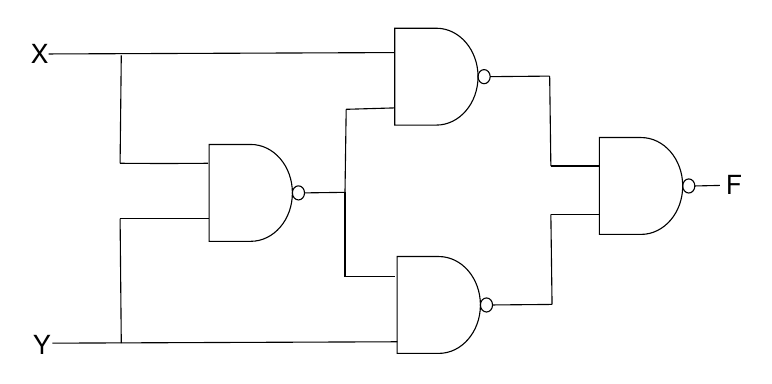
\begin{tikzpicture}[x=0.43pt,y=0.5pt,yscale=-1,xscale=1]
% Your original TikZ code here
\tikzset{every picture/.style={line width=0.75pt}} %set default line width to 0.75pt        

%Straight Lines [id:da8870235423908663] 
\draw    (99.2,109.6) -- (136.21,109.78) -- (173.2,109.6) ;
%Flowchart: Delay [id:dp3076178503272544] 
\draw   (174,96) -- (209,96) .. controls (228.33,96) and (244,111.67) .. (244,131) .. controls (244,150.33) and (228.33,166) .. (209,166) -- (174,166) -- cycle ;
%Straight Lines [id:da4880418888531195] 
\draw    (99.2,149.6) -- (111.2,149.6) -- (166.2,149.6) -- (174.2,149.6) ;
%Shape: Circle [id:dp4693486828792446] 
\draw   (244,131) .. controls (244,128.18) and (246.28,125.9) .. (249.1,125.9) .. controls (251.92,125.9) and (254.2,128.18) .. (254.2,131) .. controls (254.2,133.82) and (251.92,136.1) .. (249.1,136.1) .. controls (246.28,136.1) and (244,133.82) .. (244,131) -- cycle ;
%Straight Lines [id:da4653941185722381] 
\draw    (254.2,131) -- (288.2,130.6) ;
%Straight Lines [id:da8761511817778416] 
\draw    (39.2,30.6) -- (329.2,29.6) ;
%Straight Lines [id:da1606414736134072] 
\draw    (42.2,239.6) -- (332.2,238.6) ;
%Straight Lines [id:da6304107801712311] 
\draw    (288.2,130.6) -- (289.2,70.6) ;
%Straight Lines [id:da9368244337166334] 
\draw    (289.2,70.6) -- (329.2,69.6) ;
%Straight Lines [id:da8466357262704003] 
\draw    (288.2,191.6) -- (288.2,130.6) ;
%Straight Lines [id:da46784195426353525] 
\draw    (288.2,191.6) -- (330.2,191.6) ;
%Flowchart: Delay [id:dp9030516796824679] 
\draw   (330,12) -- (365,12) .. controls (384.33,12) and (400,27.67) .. (400,47) .. controls (400,66.33) and (384.33,82) .. (365,82) -- (330,82) -- cycle ;
%Flowchart: Delay [id:dp09252224992976132] 
\draw   (332,177) -- (367,177) .. controls (386.33,177) and (402,192.67) .. (402,212) .. controls (402,231.33) and (386.33,247) .. (367,247) -- (332,247) -- cycle ;
%Shape: Circle [id:dp5499693136350294] 
\draw   (402,212) .. controls (402,209.18) and (404.28,206.9) .. (407.1,206.9) .. controls (409.92,206.9) and (412.2,209.18) .. (412.2,212) .. controls (412.2,214.82) and (409.92,217.1) .. (407.1,217.1) .. controls (404.28,217.1) and (402,214.82) .. (402,212) -- cycle ;
%Shape: Circle [id:dp74153314191801] 
\draw   (400,47) .. controls (400,44.18) and (402.28,41.9) .. (405.1,41.9) .. controls (407.92,41.9) and (410.2,44.18) .. (410.2,47) .. controls (410.2,49.82) and (407.92,52.1) .. (405.1,52.1) .. controls (402.28,52.1) and (400,49.82) .. (400,47) -- cycle ;
%Straight Lines [id:da35345529297391987] 
\draw    (410.2,47) -- (460.2,46.6) ;
%Straight Lines [id:da8140464066015929] 
\draw    (412.2,212) -- (462.2,211.6) ;
%Flowchart: Delay [id:dp21989758956535077] 
\draw   (502,91) -- (537,91) .. controls (556.33,91) and (572,106.67) .. (572,126) .. controls (572,145.33) and (556.33,161) .. (537,161) -- (502,161) -- cycle ;
%Straight Lines [id:da14664335527509076] 
\draw    (460.2,46.6) -- (461.2,111.6) ;
%Straight Lines [id:da5388257463322341] 
\draw    (461.2,146.6) -- (462.2,211.6) ;
%Straight Lines [id:da4857250526271579] 
\draw    (461.2,111.6) -- (502.2,111.6) ;
%Straight Lines [id:da5555292815908546] 
\draw    (461.2,146.6) -- (502.2,146.6) ;
%Shape: Circle [id:dp793166461459196] 
\draw   (572,126) .. controls (572,123.18) and (574.28,120.9) .. (577.1,120.9) .. controls (579.92,120.9) and (582.2,123.18) .. (582.2,126) .. controls (582.2,128.82) and (579.92,131.1) .. (577.1,131.1) .. controls (574.28,131.1) and (572,128.82) .. (572,126) -- cycle ;
%Straight Lines [id:da6138015275286377] 
\draw    (582.2,126) -- (603.2,125.6) ;
%Straight Lines [id:da6694995059558879] 
\draw    (99.2,109.6) -- (100.2,31.6) ;
%Straight Lines [id:da9757039240740732] 
\draw    (100.2,239.6) -- (99.2,149.6) ;

% Text Node
\draw (22,22) node [anchor=north west][inner sep=0.75pt]   [align=left] {X};
% Text Node
\draw (24,232) node [anchor=north west][inner sep=0.75pt]   [align=left] {Y};
% Text Node
\draw (606,117) node [anchor=north west][inner sep=0.75pt]   [align=left] {F};


\end{tikzpicture}
     \section{Components}
     \begin{tabularx}{0.4\textwidth} { 
  | >{\centering\arraybackslash}X 
  | >{\centering\arraybackslash}X 
  | >{\centering\arraybackslash}X
  | >{\centering\arraybackslash}X | }
\hline
\textbf{Component}& \textbf{Values} & \textbf{Quantity}\\
\hline
Arduino & UNO & 1 \\  
\hline
JumperWires & M-M & 4 \\ 
\hline
LED & &3\\
\hline
     \end{tabularx}
   \section{Truth Table}
 \begin{tabularx}{0.46\textwidth} { 
  | >{\centering\arraybackslash}X
  | >{\centering\arraybackslash}X
  | >{\centering\arraybackslash}X  | }


\hline
\textbf{X} & \textbf{Y} & \textbf{OUTPUT} \\ 
\hline
0 & 0 & 0 \\
\hline
0 & 1 & 1\\
\hline
1 & 0 & 1\\
\hline
1 & 1 & 0\\
\hline
\end{tabularx}

 \begin{figure}
\centering
\includegraphics[width=0.8\columnwidth]{figs/led1(1).jpg}
\caption{led1}
\label{fig:led}
\end{figure}

\section{Implementation}
  \begin{tabularx}{0.46\textwidth} { 
  | >{\centering\arraybackslash}X 
  | >{\centering\arraybackslash}X  | }

\hline
\textbf{Arduino PIN} & \textbf{led } \\ 
\hline
D4 & INPUT \\
\hline
D5 & INPUT \\
\hline
D8 & OUTPUT \\
\hline
GND & GND \\
\hline
\end{tabularx}

\begin{center}
    Connections
\end{center}
\paragraph{Procedure}
    
    1. Connect the circuit as per the above table.\\
    2. Connect the leds to Arduino. \\
\\ \begin{tabularx}{0.57\textwidth} { 
  | >{\centering\arraybackslash}X |}
  \hline
https://github.com/MASEEDUNITIN/fwc/blob/main
/platformio/code/code.cpp\\
  \hline
\end{tabularx}


\section{Led output}[H]
\begin{figure}
\centering
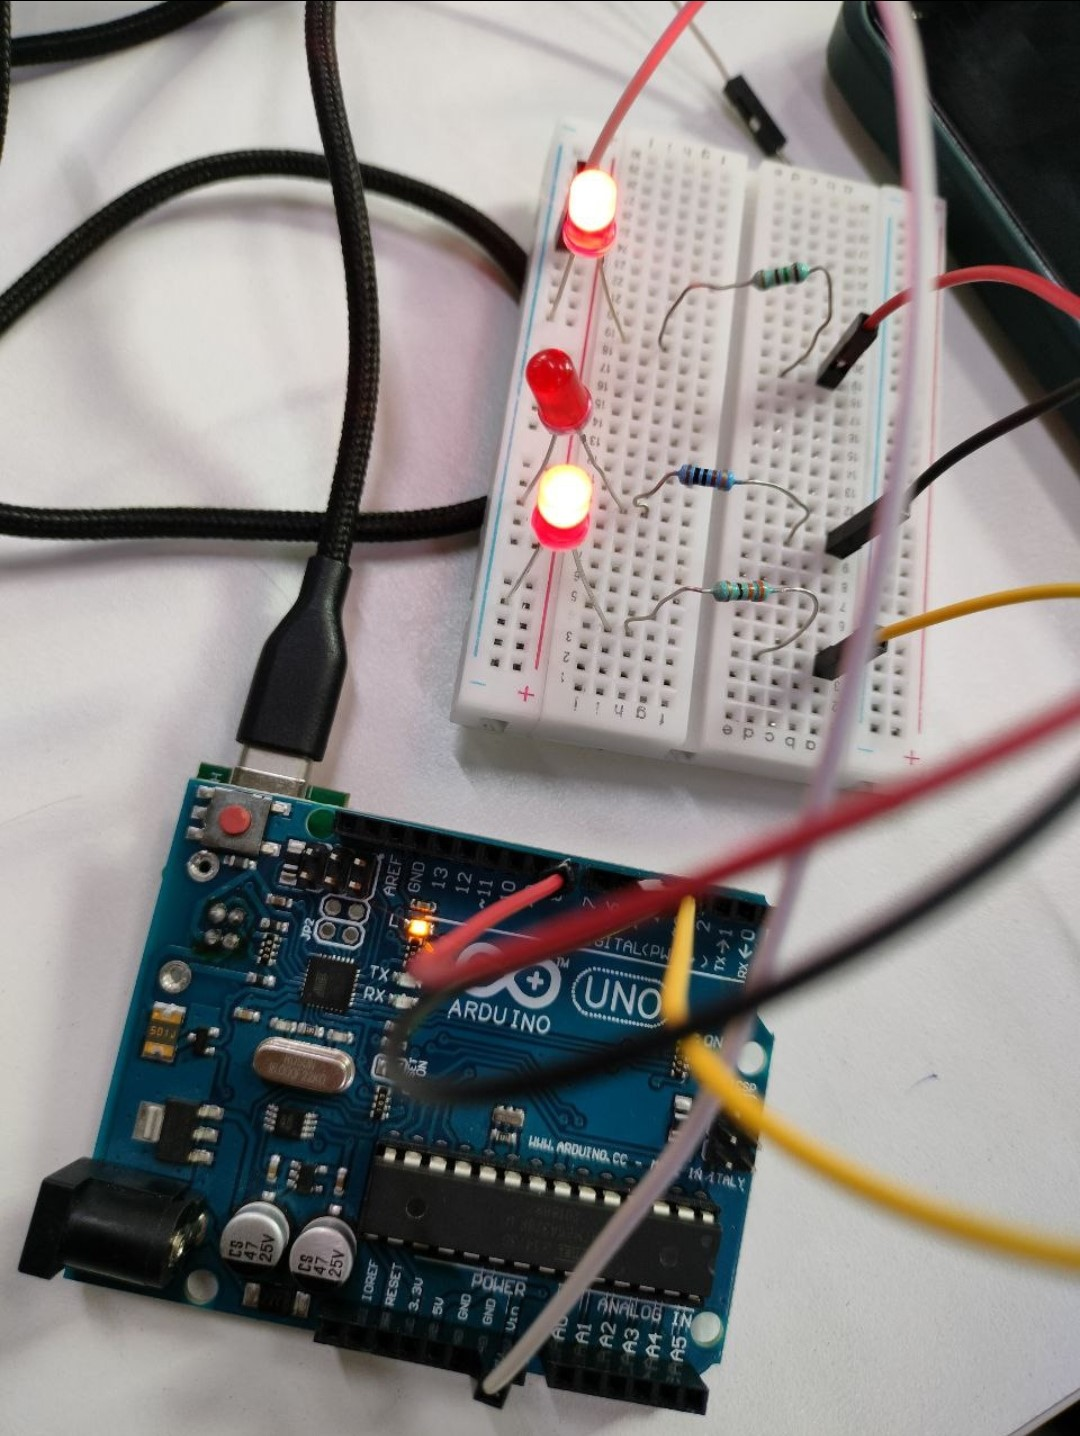
\includegraphics[width=\columnwidth]{figs/led.jpg}
\caption{Arduino connection with led}
\label{fig:led}
\end{figure}
 \bibliographystyle{ieeetr}
\end{document}
